
% Default to the notebook output style

    


% Inherit from the specified cell style.




    
\documentclass[11pt]{article}

    
    
    \usepackage[T1]{fontenc}
    % Nicer default font (+ math font) than Computer Modern for most use cases
    \usepackage{mathpazo}

    % Basic figure setup, for now with no caption control since it's done
    % automatically by Pandoc (which extracts ![](path) syntax from Markdown).
    \usepackage{graphicx}
    % We will generate all images so they have a width \maxwidth. This means
    % that they will get their normal width if they fit onto the page, but
    % are scaled down if they would overflow the margins.
    \makeatletter
    \def\maxwidth{\ifdim\Gin@nat@width>\linewidth\linewidth
    \else\Gin@nat@width\fi}
    \makeatother
    \let\Oldincludegraphics\includegraphics
    % Set max figure width to be 80% of text width, for now hardcoded.
    \renewcommand{\includegraphics}[1]{\Oldincludegraphics[width=.8\maxwidth]{#1}}
    % Ensure that by default, figures have no caption (until we provide a
    % proper Figure object with a Caption API and a way to capture that
    % in the conversion process - todo).
    \usepackage{caption}
    \DeclareCaptionLabelFormat{nolabel}{}
    \captionsetup{labelformat=nolabel}

    \usepackage{adjustbox} % Used to constrain images to a maximum size 
    \usepackage{xcolor} % Allow colors to be defined
    \usepackage{enumerate} % Needed for markdown enumerations to work
    \usepackage{geometry} % Used to adjust the document margins
    \usepackage{amsmath} % Equations
    \usepackage{amssymb} % Equations
    \usepackage{textcomp} % defines textquotesingle
    % Hack from http://tex.stackexchange.com/a/47451/13684:
    \AtBeginDocument{%
        \def\PYZsq{\textquotesingle}% Upright quotes in Pygmentized code
    }
    \usepackage{upquote} % Upright quotes for verbatim code
    \usepackage{eurosym} % defines \euro
    \usepackage[mathletters]{ucs} % Extended unicode (utf-8) support
    \usepackage[utf8x]{inputenc} % Allow utf-8 characters in the tex document
    \usepackage{fancyvrb} % verbatim replacement that allows latex
    \usepackage{grffile} % extends the file name processing of package graphics 
                         % to support a larger range 
    % The hyperref package gives us a pdf with properly built
    % internal navigation ('pdf bookmarks' for the table of contents,
    % internal cross-reference links, web links for URLs, etc.)
    \usepackage{hyperref}
    \usepackage{longtable} % longtable support required by pandoc >1.10
    \usepackage{booktabs}  % table support for pandoc > 1.12.2
    \usepackage[inline]{enumitem} % IRkernel/repr support (it uses the enumerate* environment)
    \usepackage[normalem]{ulem} % ulem is needed to support strikethroughs (\sout)
                                % normalem makes italics be italics, not underlines
    

    
    
    % Colors for the hyperref package
    \definecolor{urlcolor}{rgb}{0,.145,.698}
    \definecolor{linkcolor}{rgb}{.71,0.21,0.01}
    \definecolor{citecolor}{rgb}{.12,.54,.11}

    % ANSI colors
    \definecolor{ansi-black}{HTML}{3E424D}
    \definecolor{ansi-black-intense}{HTML}{282C36}
    \definecolor{ansi-red}{HTML}{E75C58}
    \definecolor{ansi-red-intense}{HTML}{B22B31}
    \definecolor{ansi-green}{HTML}{00A250}
    \definecolor{ansi-green-intense}{HTML}{007427}
    \definecolor{ansi-yellow}{HTML}{DDB62B}
    \definecolor{ansi-yellow-intense}{HTML}{B27D12}
    \definecolor{ansi-blue}{HTML}{208FFB}
    \definecolor{ansi-blue-intense}{HTML}{0065CA}
    \definecolor{ansi-magenta}{HTML}{D160C4}
    \definecolor{ansi-magenta-intense}{HTML}{A03196}
    \definecolor{ansi-cyan}{HTML}{60C6C8}
    \definecolor{ansi-cyan-intense}{HTML}{258F8F}
    \definecolor{ansi-white}{HTML}{C5C1B4}
    \definecolor{ansi-white-intense}{HTML}{A1A6B2}

    % commands and environments needed by pandoc snippets
    % extracted from the output of `pandoc -s`
    \providecommand{\tightlist}{%
      \setlength{\itemsep}{0pt}\setlength{\parskip}{0pt}}
    \DefineVerbatimEnvironment{Highlighting}{Verbatim}{commandchars=\\\{\}}
    % Add ',fontsize=\small' for more characters per line
    \newenvironment{Shaded}{}{}
    \newcommand{\KeywordTok}[1]{\textcolor[rgb]{0.00,0.44,0.13}{\textbf{{#1}}}}
    \newcommand{\DataTypeTok}[1]{\textcolor[rgb]{0.56,0.13,0.00}{{#1}}}
    \newcommand{\DecValTok}[1]{\textcolor[rgb]{0.25,0.63,0.44}{{#1}}}
    \newcommand{\BaseNTok}[1]{\textcolor[rgb]{0.25,0.63,0.44}{{#1}}}
    \newcommand{\FloatTok}[1]{\textcolor[rgb]{0.25,0.63,0.44}{{#1}}}
    \newcommand{\CharTok}[1]{\textcolor[rgb]{0.25,0.44,0.63}{{#1}}}
    \newcommand{\StringTok}[1]{\textcolor[rgb]{0.25,0.44,0.63}{{#1}}}
    \newcommand{\CommentTok}[1]{\textcolor[rgb]{0.38,0.63,0.69}{\textit{{#1}}}}
    \newcommand{\OtherTok}[1]{\textcolor[rgb]{0.00,0.44,0.13}{{#1}}}
    \newcommand{\AlertTok}[1]{\textcolor[rgb]{1.00,0.00,0.00}{\textbf{{#1}}}}
    \newcommand{\FunctionTok}[1]{\textcolor[rgb]{0.02,0.16,0.49}{{#1}}}
    \newcommand{\RegionMarkerTok}[1]{{#1}}
    \newcommand{\ErrorTok}[1]{\textcolor[rgb]{1.00,0.00,0.00}{\textbf{{#1}}}}
    \newcommand{\NormalTok}[1]{{#1}}
    
    % Additional commands for more recent versions of Pandoc
    \newcommand{\ConstantTok}[1]{\textcolor[rgb]{0.53,0.00,0.00}{{#1}}}
    \newcommand{\SpecialCharTok}[1]{\textcolor[rgb]{0.25,0.44,0.63}{{#1}}}
    \newcommand{\VerbatimStringTok}[1]{\textcolor[rgb]{0.25,0.44,0.63}{{#1}}}
    \newcommand{\SpecialStringTok}[1]{\textcolor[rgb]{0.73,0.40,0.53}{{#1}}}
    \newcommand{\ImportTok}[1]{{#1}}
    \newcommand{\DocumentationTok}[1]{\textcolor[rgb]{0.73,0.13,0.13}{\textit{{#1}}}}
    \newcommand{\AnnotationTok}[1]{\textcolor[rgb]{0.38,0.63,0.69}{\textbf{\textit{{#1}}}}}
    \newcommand{\CommentVarTok}[1]{\textcolor[rgb]{0.38,0.63,0.69}{\textbf{\textit{{#1}}}}}
    \newcommand{\VariableTok}[1]{\textcolor[rgb]{0.10,0.09,0.49}{{#1}}}
    \newcommand{\ControlFlowTok}[1]{\textcolor[rgb]{0.00,0.44,0.13}{\textbf{{#1}}}}
    \newcommand{\OperatorTok}[1]{\textcolor[rgb]{0.40,0.40,0.40}{{#1}}}
    \newcommand{\BuiltInTok}[1]{{#1}}
    \newcommand{\ExtensionTok}[1]{{#1}}
    \newcommand{\PreprocessorTok}[1]{\textcolor[rgb]{0.74,0.48,0.00}{{#1}}}
    \newcommand{\AttributeTok}[1]{\textcolor[rgb]{0.49,0.56,0.16}{{#1}}}
    \newcommand{\InformationTok}[1]{\textcolor[rgb]{0.38,0.63,0.69}{\textbf{\textit{{#1}}}}}
    \newcommand{\WarningTok}[1]{\textcolor[rgb]{0.38,0.63,0.69}{\textbf{\textit{{#1}}}}}
    
    
    % Define a nice break command that doesn't care if a line doesn't already
    % exist.
    \def\br{\hspace*{\fill} \\* }
    % Math Jax compatability definitions
    \def\gt{>}
    \def\lt{<}
    % Document parameters
    \title{Possible exam questions}
    
    
    

    % Pygments definitions
    
\makeatletter
\def\PY@reset{\let\PY@it=\relax \let\PY@bf=\relax%
    \let\PY@ul=\relax \let\PY@tc=\relax%
    \let\PY@bc=\relax \let\PY@ff=\relax}
\def\PY@tok#1{\csname PY@tok@#1\endcsname}
\def\PY@toks#1+{\ifx\relax#1\empty\else%
    \PY@tok{#1}\expandafter\PY@toks\fi}
\def\PY@do#1{\PY@bc{\PY@tc{\PY@ul{%
    \PY@it{\PY@bf{\PY@ff{#1}}}}}}}
\def\PY#1#2{\PY@reset\PY@toks#1+\relax+\PY@do{#2}}

\expandafter\def\csname PY@tok@w\endcsname{\def\PY@tc##1{\textcolor[rgb]{0.73,0.73,0.73}{##1}}}
\expandafter\def\csname PY@tok@c\endcsname{\let\PY@it=\textit\def\PY@tc##1{\textcolor[rgb]{0.25,0.50,0.50}{##1}}}
\expandafter\def\csname PY@tok@cp\endcsname{\def\PY@tc##1{\textcolor[rgb]{0.74,0.48,0.00}{##1}}}
\expandafter\def\csname PY@tok@k\endcsname{\let\PY@bf=\textbf\def\PY@tc##1{\textcolor[rgb]{0.00,0.50,0.00}{##1}}}
\expandafter\def\csname PY@tok@kp\endcsname{\def\PY@tc##1{\textcolor[rgb]{0.00,0.50,0.00}{##1}}}
\expandafter\def\csname PY@tok@kt\endcsname{\def\PY@tc##1{\textcolor[rgb]{0.69,0.00,0.25}{##1}}}
\expandafter\def\csname PY@tok@o\endcsname{\def\PY@tc##1{\textcolor[rgb]{0.40,0.40,0.40}{##1}}}
\expandafter\def\csname PY@tok@ow\endcsname{\let\PY@bf=\textbf\def\PY@tc##1{\textcolor[rgb]{0.67,0.13,1.00}{##1}}}
\expandafter\def\csname PY@tok@nb\endcsname{\def\PY@tc##1{\textcolor[rgb]{0.00,0.50,0.00}{##1}}}
\expandafter\def\csname PY@tok@nf\endcsname{\def\PY@tc##1{\textcolor[rgb]{0.00,0.00,1.00}{##1}}}
\expandafter\def\csname PY@tok@nc\endcsname{\let\PY@bf=\textbf\def\PY@tc##1{\textcolor[rgb]{0.00,0.00,1.00}{##1}}}
\expandafter\def\csname PY@tok@nn\endcsname{\let\PY@bf=\textbf\def\PY@tc##1{\textcolor[rgb]{0.00,0.00,1.00}{##1}}}
\expandafter\def\csname PY@tok@ne\endcsname{\let\PY@bf=\textbf\def\PY@tc##1{\textcolor[rgb]{0.82,0.25,0.23}{##1}}}
\expandafter\def\csname PY@tok@nv\endcsname{\def\PY@tc##1{\textcolor[rgb]{0.10,0.09,0.49}{##1}}}
\expandafter\def\csname PY@tok@no\endcsname{\def\PY@tc##1{\textcolor[rgb]{0.53,0.00,0.00}{##1}}}
\expandafter\def\csname PY@tok@nl\endcsname{\def\PY@tc##1{\textcolor[rgb]{0.63,0.63,0.00}{##1}}}
\expandafter\def\csname PY@tok@ni\endcsname{\let\PY@bf=\textbf\def\PY@tc##1{\textcolor[rgb]{0.60,0.60,0.60}{##1}}}
\expandafter\def\csname PY@tok@na\endcsname{\def\PY@tc##1{\textcolor[rgb]{0.49,0.56,0.16}{##1}}}
\expandafter\def\csname PY@tok@nt\endcsname{\let\PY@bf=\textbf\def\PY@tc##1{\textcolor[rgb]{0.00,0.50,0.00}{##1}}}
\expandafter\def\csname PY@tok@nd\endcsname{\def\PY@tc##1{\textcolor[rgb]{0.67,0.13,1.00}{##1}}}
\expandafter\def\csname PY@tok@s\endcsname{\def\PY@tc##1{\textcolor[rgb]{0.73,0.13,0.13}{##1}}}
\expandafter\def\csname PY@tok@sd\endcsname{\let\PY@it=\textit\def\PY@tc##1{\textcolor[rgb]{0.73,0.13,0.13}{##1}}}
\expandafter\def\csname PY@tok@si\endcsname{\let\PY@bf=\textbf\def\PY@tc##1{\textcolor[rgb]{0.73,0.40,0.53}{##1}}}
\expandafter\def\csname PY@tok@se\endcsname{\let\PY@bf=\textbf\def\PY@tc##1{\textcolor[rgb]{0.73,0.40,0.13}{##1}}}
\expandafter\def\csname PY@tok@sr\endcsname{\def\PY@tc##1{\textcolor[rgb]{0.73,0.40,0.53}{##1}}}
\expandafter\def\csname PY@tok@ss\endcsname{\def\PY@tc##1{\textcolor[rgb]{0.10,0.09,0.49}{##1}}}
\expandafter\def\csname PY@tok@sx\endcsname{\def\PY@tc##1{\textcolor[rgb]{0.00,0.50,0.00}{##1}}}
\expandafter\def\csname PY@tok@m\endcsname{\def\PY@tc##1{\textcolor[rgb]{0.40,0.40,0.40}{##1}}}
\expandafter\def\csname PY@tok@gh\endcsname{\let\PY@bf=\textbf\def\PY@tc##1{\textcolor[rgb]{0.00,0.00,0.50}{##1}}}
\expandafter\def\csname PY@tok@gu\endcsname{\let\PY@bf=\textbf\def\PY@tc##1{\textcolor[rgb]{0.50,0.00,0.50}{##1}}}
\expandafter\def\csname PY@tok@gd\endcsname{\def\PY@tc##1{\textcolor[rgb]{0.63,0.00,0.00}{##1}}}
\expandafter\def\csname PY@tok@gi\endcsname{\def\PY@tc##1{\textcolor[rgb]{0.00,0.63,0.00}{##1}}}
\expandafter\def\csname PY@tok@gr\endcsname{\def\PY@tc##1{\textcolor[rgb]{1.00,0.00,0.00}{##1}}}
\expandafter\def\csname PY@tok@ge\endcsname{\let\PY@it=\textit}
\expandafter\def\csname PY@tok@gs\endcsname{\let\PY@bf=\textbf}
\expandafter\def\csname PY@tok@gp\endcsname{\let\PY@bf=\textbf\def\PY@tc##1{\textcolor[rgb]{0.00,0.00,0.50}{##1}}}
\expandafter\def\csname PY@tok@go\endcsname{\def\PY@tc##1{\textcolor[rgb]{0.53,0.53,0.53}{##1}}}
\expandafter\def\csname PY@tok@gt\endcsname{\def\PY@tc##1{\textcolor[rgb]{0.00,0.27,0.87}{##1}}}
\expandafter\def\csname PY@tok@err\endcsname{\def\PY@bc##1{\setlength{\fboxsep}{0pt}\fcolorbox[rgb]{1.00,0.00,0.00}{1,1,1}{\strut ##1}}}
\expandafter\def\csname PY@tok@kc\endcsname{\let\PY@bf=\textbf\def\PY@tc##1{\textcolor[rgb]{0.00,0.50,0.00}{##1}}}
\expandafter\def\csname PY@tok@kd\endcsname{\let\PY@bf=\textbf\def\PY@tc##1{\textcolor[rgb]{0.00,0.50,0.00}{##1}}}
\expandafter\def\csname PY@tok@kn\endcsname{\let\PY@bf=\textbf\def\PY@tc##1{\textcolor[rgb]{0.00,0.50,0.00}{##1}}}
\expandafter\def\csname PY@tok@kr\endcsname{\let\PY@bf=\textbf\def\PY@tc##1{\textcolor[rgb]{0.00,0.50,0.00}{##1}}}
\expandafter\def\csname PY@tok@bp\endcsname{\def\PY@tc##1{\textcolor[rgb]{0.00,0.50,0.00}{##1}}}
\expandafter\def\csname PY@tok@fm\endcsname{\def\PY@tc##1{\textcolor[rgb]{0.00,0.00,1.00}{##1}}}
\expandafter\def\csname PY@tok@vc\endcsname{\def\PY@tc##1{\textcolor[rgb]{0.10,0.09,0.49}{##1}}}
\expandafter\def\csname PY@tok@vg\endcsname{\def\PY@tc##1{\textcolor[rgb]{0.10,0.09,0.49}{##1}}}
\expandafter\def\csname PY@tok@vi\endcsname{\def\PY@tc##1{\textcolor[rgb]{0.10,0.09,0.49}{##1}}}
\expandafter\def\csname PY@tok@vm\endcsname{\def\PY@tc##1{\textcolor[rgb]{0.10,0.09,0.49}{##1}}}
\expandafter\def\csname PY@tok@sa\endcsname{\def\PY@tc##1{\textcolor[rgb]{0.73,0.13,0.13}{##1}}}
\expandafter\def\csname PY@tok@sb\endcsname{\def\PY@tc##1{\textcolor[rgb]{0.73,0.13,0.13}{##1}}}
\expandafter\def\csname PY@tok@sc\endcsname{\def\PY@tc##1{\textcolor[rgb]{0.73,0.13,0.13}{##1}}}
\expandafter\def\csname PY@tok@dl\endcsname{\def\PY@tc##1{\textcolor[rgb]{0.73,0.13,0.13}{##1}}}
\expandafter\def\csname PY@tok@s2\endcsname{\def\PY@tc##1{\textcolor[rgb]{0.73,0.13,0.13}{##1}}}
\expandafter\def\csname PY@tok@sh\endcsname{\def\PY@tc##1{\textcolor[rgb]{0.73,0.13,0.13}{##1}}}
\expandafter\def\csname PY@tok@s1\endcsname{\def\PY@tc##1{\textcolor[rgb]{0.73,0.13,0.13}{##1}}}
\expandafter\def\csname PY@tok@mb\endcsname{\def\PY@tc##1{\textcolor[rgb]{0.40,0.40,0.40}{##1}}}
\expandafter\def\csname PY@tok@mf\endcsname{\def\PY@tc##1{\textcolor[rgb]{0.40,0.40,0.40}{##1}}}
\expandafter\def\csname PY@tok@mh\endcsname{\def\PY@tc##1{\textcolor[rgb]{0.40,0.40,0.40}{##1}}}
\expandafter\def\csname PY@tok@mi\endcsname{\def\PY@tc##1{\textcolor[rgb]{0.40,0.40,0.40}{##1}}}
\expandafter\def\csname PY@tok@il\endcsname{\def\PY@tc##1{\textcolor[rgb]{0.40,0.40,0.40}{##1}}}
\expandafter\def\csname PY@tok@mo\endcsname{\def\PY@tc##1{\textcolor[rgb]{0.40,0.40,0.40}{##1}}}
\expandafter\def\csname PY@tok@ch\endcsname{\let\PY@it=\textit\def\PY@tc##1{\textcolor[rgb]{0.25,0.50,0.50}{##1}}}
\expandafter\def\csname PY@tok@cm\endcsname{\let\PY@it=\textit\def\PY@tc##1{\textcolor[rgb]{0.25,0.50,0.50}{##1}}}
\expandafter\def\csname PY@tok@cpf\endcsname{\let\PY@it=\textit\def\PY@tc##1{\textcolor[rgb]{0.25,0.50,0.50}{##1}}}
\expandafter\def\csname PY@tok@c1\endcsname{\let\PY@it=\textit\def\PY@tc##1{\textcolor[rgb]{0.25,0.50,0.50}{##1}}}
\expandafter\def\csname PY@tok@cs\endcsname{\let\PY@it=\textit\def\PY@tc##1{\textcolor[rgb]{0.25,0.50,0.50}{##1}}}

\def\PYZbs{\char`\\}
\def\PYZus{\char`\_}
\def\PYZob{\char`\{}
\def\PYZcb{\char`\}}
\def\PYZca{\char`\^}
\def\PYZam{\char`\&}
\def\PYZlt{\char`\<}
\def\PYZgt{\char`\>}
\def\PYZsh{\char`\#}
\def\PYZpc{\char`\%}
\def\PYZdl{\char`\$}
\def\PYZhy{\char`\-}
\def\PYZsq{\char`\'}
\def\PYZdq{\char`\"}
\def\PYZti{\char`\~}
% for compatibility with earlier versions
\def\PYZat{@}
\def\PYZlb{[}
\def\PYZrb{]}
\makeatother


    % Exact colors from NB
    \definecolor{incolor}{rgb}{0.0, 0.0, 0.5}
    \definecolor{outcolor}{rgb}{0.545, 0.0, 0.0}



    
    % Prevent overflowing lines due to hard-to-break entities
    \sloppy 
    % Setup hyperref package
    \hypersetup{
      breaklinks=true,  % so long urls are correctly broken across lines
      colorlinks=true,
      urlcolor=urlcolor,
      linkcolor=linkcolor,
      citecolor=citecolor,
      }
    % Slightly bigger margins than the latex defaults
    
    \geometry{verbose,tmargin=1in,bmargin=1in,lmargin=1in,rmargin=1in}
    
    

    \begin{document}
    
    
    \maketitle
    
    

    
    \section{Possible exam questions}\label{possible-exam-questions}

During the lectures course Paul van der Werf mentioned several possible
questions that could be asked at the exam. These are all listed below.

    \begin{itemize}
\tightlist
\item
  \textbf{What is the difference between detailed balance and
  statistical equilibrium?} (Lecture 2, hour 1)
\end{itemize}

\textbf{Answer} Detailed balance means every process is balanced by its
counterproces. Statistical equilbrium means that sum of the rates of all
processes populating level \(i\) equals the sum of rates of all
processes depopulating the level \(i\). So, the difference is that in
statistical equilbrium the \emph{sum} of the processes considered, it
does not saying anything about a process and its counterprocess.

    \begin{itemize}
\tightlist
\item
  \textbf{Why is \(I_\nu\) an intrinsic property of a source, and
  \(F_\nu\) not?} (Lecture 2, hour 1) (Not really an exam question but
  would be nice to understand).
\end{itemize}

\textbf{Answer}: The specific intensity defines the directional value of
the radiation field and is defined per unit of solid angle. The flux is
the specific energy integrated over the solid angle. This means the
distance independence is eliminated.

    \begin{itemize}
\tightlist
\item
  \textbf{Why doe sthe factor 1 over the speed of light emergy in the
  definition of the specific energy density?} (Lecture 2, hour 1)
\end{itemize}

\textbf{Answer}: Flux density has units erg s-1 cm-1 Hz-1 or Jy.
Specific energy density is defined as 1 over the speed of light times
the flux density. The units then become erg cm-2 Hz-1. So from a measure
of energy per unit of time per unit of distance, it transforms into a
unit of energy per area. This makes sense. Since energy comes in with a
velocity equal to the speed of light, you have to devide by \(c\) to
remove the time factor and obtain the energy density per area.

    \begin{itemize}
\tightlist
\item
  \textbf{What is a recombination line?} (Lecture 4, hour 2)
\end{itemize}

\textbf{Answer}: Recombination lines are spectral lines corresponding
with the energy released from the recombination of an ion with an
electron.

    \begin{itemize}
\tightlist
\item
  \textbf{Explain what case A and case B recombination means.} (Lecture
  4, hour 2)
\end{itemize}

\textbf{Answer}: \textbf{Case A}: Case A is optically thin to ionizing
radiation. This means that every ionizing photon emitted during the
recombination preocess escapes. For this case, we sum the radiative
capture rate coefficient \(\alpha_{nl}\) overa ll levels \(nl\).
\textbf{Case B}: Case B is optically thick to radiation just above
\(I_H = 13.60 \text{ eV}\), so that ionizing photons emitted during
recombination are immediatly reabsorbed, creating another ion and free
electron by photoionization. In this case, the recombinations directly
to \(n=1\) do not reduce the ionization of the gas: only recombinations
to \(n \geq 2\) act to reduce the ionizzation.

    \begin{itemize}
\tightlist
\item
  \textbf{Don't confuse recombination lines with collisionally excited
  lines, people always do that at the exam. What is the difference?}
  (Lecture 4, hour 2)
\end{itemize}

\textbf{Answer}: Recombination lines are spectral lines corresponding
with the energy released from the recombination of an ion with an
electron. Collisional excitation means that 2 particles collide
inelastically. Kinetic energy is transformed into internal energy of
particles. At least one of the particles goes to a higher quantum state.
This collision produces a spectral line that corresponds with the energy
conversion.

    \begin{itemize}
\tightlist
\item
  Discussion questions lecture 4 (hour 2):
\item
  Assume we can image Halpha and Hbeta emission from an HII region. How
  can we correct for extinction?
\item
  Does it matter whether the dust is located in a foreground absorbing
  cloud or is mixed with the ionized gas? \emph{Hint}: has to do with
  radiative transfer.
\end{itemize}

    \begin{itemize}
\tightlist
\item
  \textbf{Derive the Strömgren radius.} (Lecture 5, hour 1)
\end{itemize}

\textbf{Answer}:

The strömgren sphere is a fully ionized, spherical region of uniform
density, assuming the ionization to be maintained by absorption of the
ionizing photons radiated by a central hot star. The strömgen radius is
derived by

\[ \text{Recombination rate} = \text{Photoionization rate} \]

Let \(Q_0\) be the rate of emission of hydrogen-ionizing photons, i.e.,
\(h\nu > I_H = 13.6 \text{ eV}\)

Every radiative recombination:

\[ \text{H}^+ + e^- \rightarrow \text{H} + h\nu \]

is balanced by a photoionization:

\[ \text{H} + h\nu \rightarrow \text{H}^+ + e^- \]

The hydrogen density \(n_H\) equals the density of the ionized hydrogen
\(n(\text{H}^+)\).

Using case B radiation recombination coefficient \(\alpha_B\), the
following equation results:

\[ Q_0 = \frac{4\pi}{3} R_{S0}^3 \alpha_B n(\text{H}^+) n_e \]

Because \(n(\text{H}^+) = n_e = n_H\), we can solve for the Strömgen
radius:

\[ R_{SO} = \bigg( \frac{3 Q_0}{4 \pi n_H^2 \alpha_B} \bigg)^\frac{1}{3} \]

    \begin{itemize}
\tightlist
\item
  \textbf{Explain how recombination lines are used to determine the SFR,
  and discuss the uncertainties.} (Lecture 5, hour 2)
\end{itemize}

\textbf{Answer}: The luminosity coming from recombination lines measures
the rate of emission of hydrogen-ionizing photons, \(Q_0\) coming from
the central young hot star, assuming an HII region. It tells you what
kind of star is there. If the luminosity of recombination lines for a
whole galaxy can be measured, the formation rate of O-stars can be
deduced. O-stars are short lived stars, their lifetime w.r.t long living
stars can be neglected. Therefore the number of O stars in a galaxy is a
measure of the star formation rate (SFR) in a galaxy.

Sources of uncertainty:

\begin{enumerate}
\def\labelenumi{\arabic{enumi}.}
\tightlist
\item
  To relate the number of O-stars to the star formation rate, you need
  to assume a star formation history. For example, there are two extreme
  assumptions. One assumes a constant star formation rate, and the other
  is a sudden burst of star formation; all stars form at a particular
  moment and after that no more stars are formed. The real situation is
  somewhere in between these two extremes.
\item
  To go from the SFR of O-stars, to the SFR in general, you need to know
  the mass fraction of O-stars w.r.t all the stars. This means you need
  to assume an \emph{initial mass function}. This is a major source of
  uncertainty.
\end{enumerate}

    \begin{itemize}
\tightlist
\item
  \textbf{You need to be able to do the excitation in a 2-level system
  analysis on the exam. Maybe a 3-level system, but then it will be
  simplified. The excitation without induced radiative transitions will
  extremely likely be at the exam. So the system with the Einstein A
  coefficient and the collisional (de)-excitation arrows.} (lecture 6,
  hour 1)
\end{itemize}

\textbf{Answer}:

\begin{itemize}
\tightlist
\item
  \textbf{Spontaneous emission}: The process in which a quantum
  mechanical system transits from an excited energy state to a lower
  energy state (e.g. its ground state) and emits a quantized amount of
  energy in the form of a photon.
\end{itemize}

\[ X_u \rightarrow X_l + h\nu_{ul} \]

\[ - \frac{\text{d}n_u}{\text{d}t} = \frac{\text{d}n_l}{\text{d}t}= A_{ul}n_u \]

\begin{itemize}
\tightlist
\item
  \textbf{Absorption}: Matter taking up a photon's energy and transforms
  is into internal energy (for example, thermal energy).
\end{itemize}

\[ X_l + h\nu \rightarrow X_u \]

\[ \frac{\text{d}n_u}{\text{d}t} = - \frac{\text{d}n_l}{\text{d}t}= B_{lu}n_l \int u_\nu \phi_nu \text{d}\nu \]

\begin{itemize}
\tightlist
\item
  \textbf{Stimulated emission}: The process by which an incoming photon
  of a specific frequency can interact with an excited atomic electron,
  causing it to drop to a lower energy level.
\end{itemize}

\[ X_u + h\nu \rightarrow X_l + 2h\nu \]

\[ \frac{\text{d}n_l}{\text{d}t} = - \frac{\text{d}n_u}{\text{d}t}= B_{ul}n_u \int u_\nu \phi_nu \text{d}\nu \]

\begin{itemize}
\tightlist
\item
  \textbf{Collisional excitation}: When the temperature of IS gas
  becomes so hot, the collisions between atoms become so strong that
  they are able to ionized each other. This is called collisional
  excitation. The kinetic energy of a collision partner is converted
  into the internal energy of a reactant species. Using the collisional
  (de)excitation coefficients \(k_{01}\) and
  \(k_{10} \text{ [cm3s-1]}\), and the density \(n_c\) of the collision
  partner, we can set up the following equations for the collisional
  (de)excitation rates:
\end{itemize}

\[ C_{01} = k_{01} n_c \]

\begin{itemize}
\tightlist
\item
  \textbf{Collisional deexcitation}: The inverse process of collisional
  excitation.
\end{itemize}

\[ C_{10} = k_{10} n_c \]

Using the above excitation and deexcitation mechanism, you can set up a
2-level system:

\begin{figure}
\centering
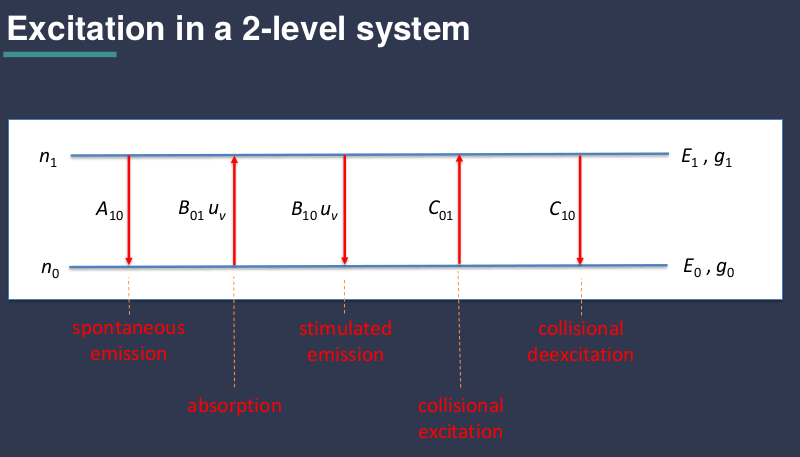
\includegraphics{figs/fig_1.png}
\caption{}
\end{figure}

The situation \textbf{Excitation without induced radiative transitions}
can be seen as a special case of the general situation sketeched in the
figure above. In this particular situation, there is no absorption and
stimulated emission; so the two arrows containing the Einstein
\(B\)-coefficient vanish. This is the case when the ISM is optically
thin, because then photons will escape instead of getting absorpted by
an atom or stimulate emission in an atom.

    \begin{itemize}
\tightlist
\item
  \textbf{Understand the criticial density and the high \& low density
  limit. Which one is dependent on density and which one is independent.
  You should be able to explain without thinking about it.} (lecture 6,
  hour 1)
\end{itemize}

\textbf{Answer}:

The critical density is defined as the ratio of the Einstein \(A\)
coefficient and the collisional deexcitation coefficient:

\[ n_\text{crit} = \frac{A_{10}}{k_{10}} \]

It is the density at which the spontaneous decay and collisional
deexcitation are equally important.

From this the following important expression and result follows:

\[ \frac{n_1}{n_0} = \frac{1}{1 + \frac{n_\text{crit}}{n_c}} \frac{g_i}{g_0} e^{-\frac{E_{10}}{kT_\text{kin}}} \]

The important implications form this are the low and high density
limits. The high density limit is:

\[ n_c >> n_\text{crit} \]

\[ \frac{n_1}{n_0} = \frac{g_i}{g_0} e^{-\frac{E_{10}}{kT_\text{kin}}} \]

\[ T_\text{ex} = T_\text{kin} \rightarrow \text{ Thermalized levels & independent of density} \]

In the low density limit:

\[ n_c << n_\text{crit} \]

\[ \frac{n_1}{n_0} = \frac{n_c}{n_\text{crit}} \frac{g_i}{g_0} e^{-\frac{E_{10}}{kT_\text{kin}}} \rightarrow \text{ Subthermal excitation & dependent on density} \]

    \begin{itemize}
\tightlist
\item
  \textbf{Application 2 is a typical exam question. Draine figures 17.4
  en 17.5. Explain the behaviour of the curves of figure 17.4.} (lecture
  6, hour 2)
\end{itemize}

\textbf{Answer}:

So in figure 17.4 there are 2 clear regimes. To the left of the critical
density \(n_\text{crit}\), and to that right of it. To the left it is
linear, and to the right they flatten. Remember that we have the two
limiting cases:

\[ n_c >> n_\text{crit} \] \[ n_c << n_\text{crit} \]

To the right of \(n_\text{crit}\), we are in the high density limit
which means the energy levels are thermalized and there is density
independence. Making the density higher does not make the levels more
thermalized. Therefore the curve flattens to the right of
\(n_\text{crit}\).

To the left of \(n_\text{crit}\) we are in the low density limit, which
means with increasing density the line ratio increases. So it is
dependent and a function of density. This is the general behaviour of an
excitation plot, because they are all governed by the same equation.

    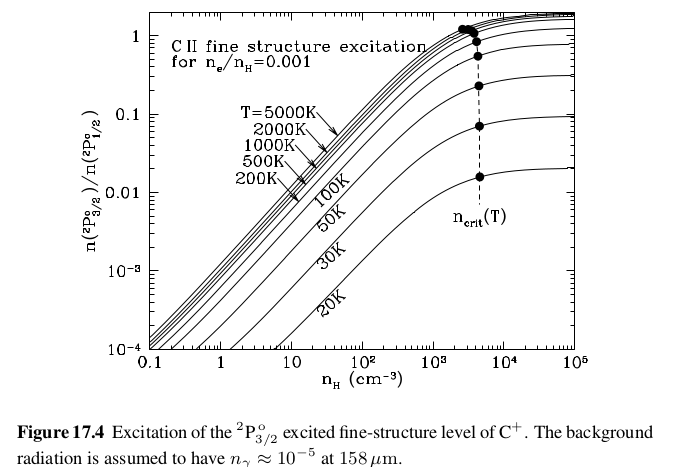
\includegraphics{figs/fig_2.png} 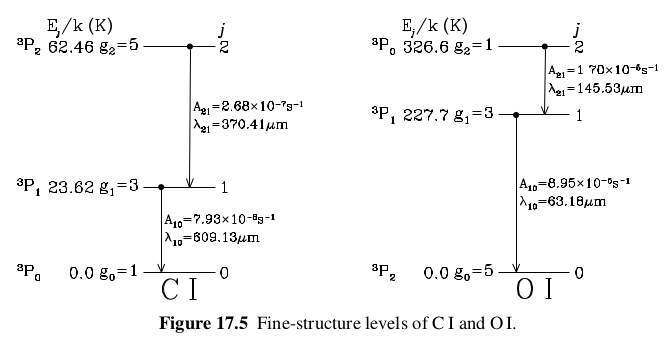
\includegraphics{figs/fig_3.png}

    \begin{itemize}
\tightlist
\item
  \textbf{Understand slide 34 of lecture 6. Explain the behaviour and
  shape of the curves.} (lecture 7, hour 1)
\end{itemize}

\begin{figure}
\centering
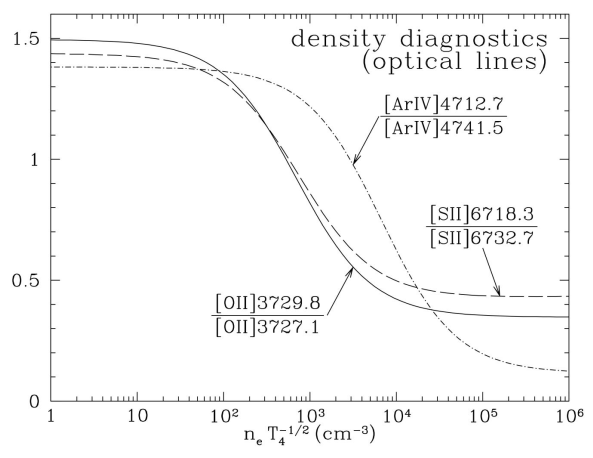
\includegraphics{figs/fig_4.png}
\caption{}
\end{figure}

    \textbf{Answer}: Line ratios as function of \(n_e\) always behave like
this, and there is a simple way to explain this. What stands out is that
in the upper left and in the lower right the line ratio is independent
of density. In the low density you are below the critical density for
both lines. For both lines the line ratio is proportional to the
density, so if you take the ratio, the density is going to drop out. So
there is no density dependence there. In the right side, you are above
the critical density. So both lines are independent of density, so the
ratio is also indepedent of density. So, only in the region between low
and high density, there is a dependence. This is also where the critical
density will be.

    \begin{itemize}
\tightlist
\item
  \textbf{Understand self-shielding. What is it, why is it important,
  when does it happen?} (Lecture 8, hour 2)
\end{itemize}

\textbf{Answer}: H\(_2\) photodissociation is a line absorption process
and if the lines get optically thick, they will shield the deeper layers
from dissociating photons. This phenomenon is known as
\emph{self-shielding}. Molecular clouds are molecular because of
self-shielding.

    \begin{itemize}
\tightlist
\item
  \textbf{Why do H2 regions always have a temperature around 8000 K?}
  (Lecture 9, hour 1)
\end{itemize}

\textbf{Answer}: At 8000 K, the photodisassociation rate equals the
cooling due to free-free cooling, recombination and collisional
excitation. You could even ignore free-free cooling and recombination
because collisional excitation is dominant. So HII regions at 8000 K are
in an equilibrium state between photodisassociation and cooling.

    \begin{itemize}
\tightlist
\item
  \textbf{Why is dust emission not a cooling mechanism of gas?} (Lecture
  9, hour 1)
\end{itemize}

\textbf{Answer}: It cools the dust, not the gas. This means that dust
and the gas are not thermally coupled; they are two separate
thermodynamic systems. Only at high densities, dust and gas become
thermally coupled and the temperatures become the same.

    \begin{itemize}
\tightlist
\item
  \textbf{Explain how collisional excitation is a cooling mechanism. How
  do we know it is the dominant cooling mechanism?} (Lecture 9, hour 1)
\end{itemize}

\textbf{Answer}: You have a particle that is in the ground state, and it
gets collisionally excited to a higher internal state. This costs energy
which comes from kinetic energy of the colliding system. After that
there is radiative decay, which sends out a photon. This is a cooling
mechanism. So the line emission we observe is really a cooling
mechanism. We know collisional excitation is the dominant cooling
mechanism because of the following reasoning. If a metal-free HII region
is considered, and we apply the physics only of recombination lines and
free-free cooling, a temperature of HII regions would have approximately
the same temperature of their central stars (20000 - 50000 K). This is
not what we observe. If cooling by collisional excitation is taken into
account, you end up with temperatures from 6000 to 10000 K. This is what
we observe, therefore we know that this is the dominant cooling
mechanism.

    \begin{itemize}
\tightlist
\item
  \textbf{Why does the temperature increase with density for HII
  regions?} (Lecture 9, hour 1, at the end) (typical exam question)
\end{itemize}

\textbf{Answer}: The next collision happens before photo-emission.
Because of that the gas can't cool and the temperature rises.

    \begin{itemize}
\tightlist
\item
  \textbf{5 times during the lectures the 2-phase ISM was mentioned as a
  potential exam question. Therefore it is extremely likely this will be
  on the exam.}
\end{itemize}

{[}1{]} \textbf{Explain the observational evidence for the 2-phase ISM
(The cold neutral medium and the hot neutral medium)}. (Lecture 3, hour
2) (Lecture 4, hour 1).

{[}2{]} \textbf{Explain why there is a cold neutral medium and a warm
neutral medium, with two different temperatures.} (Lecture 9, hour 1)

{[}3{]} \textbf{Make sure to be able to explain the physical meaning of
figure 30.2b of Draine. Be able to sketch it, indicate net heating and
cooling, and explain the existence of the 2-phase atomic medium.}
(Lecture 9, hour 2)

{[}4{]} \textbf{What is the observational evidence and what is the
theoretical explanation for it? To be explained without any equations.}
(Lecture 12, hour 2)

\begin{figure}
\centering
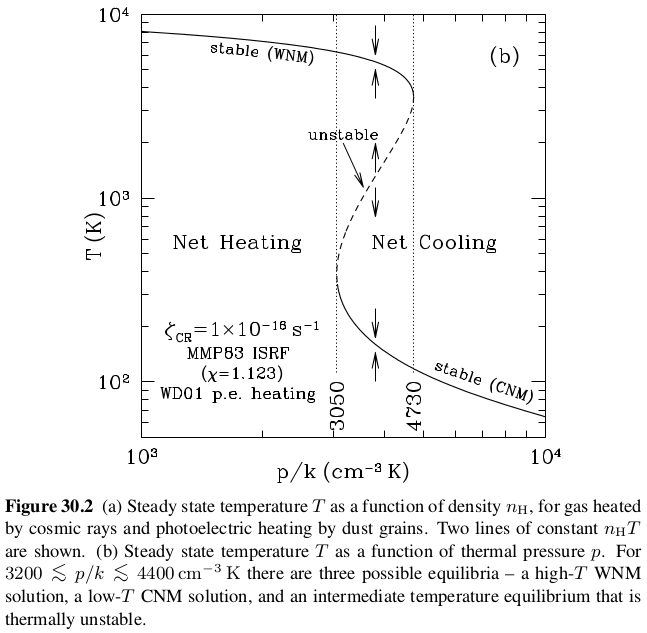
\includegraphics{figs/fig_5.png}
\caption{}
\end{figure}

    \textbf{Answer}: The figure provides the theoretical explanation for the
existence of the 2-phase ISM. In the above figure, the vertical axis
displays the y-axis and the horizontal axis the pressure. The curve is
the equilibrium between heating and cooling. So you pick a pressure and
then you read of the equilibrium temperature, with the pressure being
the product of density and temperature. To the right of the curve there
is more cooling than heating, and to the left there is more heating then
cooling. It turns out that the pressure of the WNM in the MW has a
pressure in the range in the middle; so the range between 3050
cm\(^{-3}\)K en 4730 cm\(^{-3}\)K, where there are three theoretical
temperature values. So at approximately 4000 cm\(^{-3}\)K, there is the
CNM at 150 K and the WNM at 5000 K. In pressure equilibrium of course,
or else the gas would start moving. There is also a third solution at
about 1000 K. However, this solution is unstable. This means if you
perturb the solution, you will further away from the curve until you
reach a stable part of the curve. An increase in pressure will set in
motion the cooling until the stable solution is reached. So there are
two solutions, the CNM and WNM. This is one of the nicest thing of
interstellar medium physics. We produce the physics that we observe.

For the observational evidence: A warm cloud is optically thin and
\(T_b\) scales with the column density as long as the line is optically
thin. A Cold cloud is optically thick no matter how large the column
density is. So emission is dominated by the WNM and absorption by the
CNM. The CNM have \(T_\text{kin}\) around 80 K and cause the narrow
emission peaks and the absoprtions. The WNM is an extended warm medium
the causes the borad emission features without detectable absorption.
The temperature is hard to determine, but is somewhere around 8000 K.

    \begin{itemize}
\tightlist
\item
  \textbf{Why is direct measurement of molecular hydrogen mass so
  difficult?.} (Lecture 10, hour 1)
\end{itemize}

\textbf{Answer}:


    % Add a bibliography block to the postdoc
    
    
    
    \end{document}
